
%(BEGIN_QUESTION)
% Copyright 2011, Tony R. Kuphaldt, released under the Creative Commons Attribution License (v 1.0)
% This means you may do almost anything with this work of mine, so long as you give me proper credit

En analysator som måler konsentrasjonen av svoveldioksid (SO$_2$) i avgassen fra en stor forbrenningsovn krever at sensortemperaturen styres svært nøyaktig. I denne analysatoren reguleres temperaturen av en analog op-amp-basert regulatorkrets. Temperaturen måles med en NTC-termistor (1500 ohm ved romtemperatur, med synkende resistans ved økende temperatur). Varme tilføres sensorhuset av et 75 watt varmeelement styrt av den analoge kretsen:

$$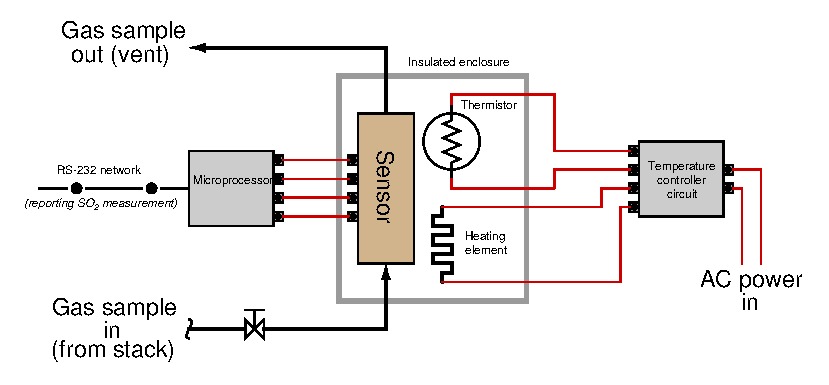
\includegraphics[width=15.5cm]{i01210x01.eps}$$

Etter mange års drift viser det seg at levetiden til den kostbare analyzersensoren kan økes betydelig ved høyere driftstemperatur, uten at målenøyaktigheten på SO$_2$ reduseres. Du blir bedt om å heve settpunktet i temperaturregulatoren, men oppdager at regulatoren er helt uten justeringsmuligheter. Den har ikke settpunktsjustering, og alle komponenter er innstøpt i epoksy, slik at kretskomponenter ikke kan byttes.

\vskip 10pt

Foreslå en løsning som gjør at temperaturreguleringen opererer ved høyere temperatur, men fortsatt kompenserer fullt ut for endringer i omgivelsestemperatur. Vær så detaljert som nødvendig.

\underbar{file i01210}
%(END_QUESTION)





%(BEGIN_ANSWER)

Et fullgodt svar fungerer under alle forhold, mens et halvgodt svar bare fungerer i enkelte situasjoner.

\vskip 10pt

Eksempel på full uttelling: en forklaring av hvordan termistorkretsen kan endres slik at den registrerer høyere resistans ved samme temperatur som før (slik at regulatoren ``tror'' sensoren er kaldere og dermed regulerer mot et høyere effektivt settpunkt).

Eksempel på halv uttelling: forslag om å øke varmeeffekten (f.eks. mer isolasjon rundt huset eller kraftigere varmeelement) gir bare delvis uttelling, fordi regulatoren etter hvert vil kompensere.

Eksempel på halv uttelling: å foreslå å bytte termistor uten å spesifisere egenskapene til ny termistor (for eksempel at den må ha høyere resistans ved samme temperatur enn den gamle).

%(END_ANSWER)





%(BEGIN_NOTES)

{\bf Denne oppgaven er kun ment for prøver/eksamen, ikke arbeidsark!}

%(END_NOTES)

